\documentclass[11pt]{article}
\usepackage{listings}
\usepackage{graphicx}
\usepackage{subfig}

\setlength{\oddsidemargin}{0.0in}
\setlength{\evensidemargin}{0.0in}
\setlength{\topmargin}{-0.25in}
\setlength{\headheight}{0in}
\setlength{\headsep}{0in}
\setlength{\textwidth}{6.5in}
\setlength{\textheight}{9.25in}
\setlength{\parindent}{0in}
\setlength{\parskip}{2mm}

\lstset{
basicstyle=\ttfamily,
numbers=left,
xleftmargin=20pt
}

\begin{document}

\section{Formatting \& Printing in SymPy}
\subsection{Features and Usage}
While SymPy’s symbolic math modules provide a fertile platform for a wide range of computational applications, the printing and formatting modules enable the results of those applications to be formatted correctly and shared easily. This is a very powerful feature facilitating mathematicians, scientists, and engineers to express the formulas of their calculations in a human readable form.

SymPy defines special terminology when it comes to printing and formatting. For starters, printing an expression is not synonymous–in the traditional sense–with printing to paper or the screen¬; instead, it means that the expression is formatted (depending on output) and returned as a standard Python string. For the more conventional definition of printing, SymPy offers a preview mode that outputs the expression as a rendered image, ready for a research report or presentation.

Printing relies on the polymorphic nature of Python to produce the correct output for any SymPy expression. To the end user, printing an expression involves just invoking the standard print function of Python. No special processing or compilation beforehand is required. The ease of use is illustrated below:

\begin{lstlisting}
>>> from sympy import Integral
>>> from sympy.abc import x
>>> print x**2
x**2
>>> print 1/x
1/x
>>> print Integral(x**2, x)
Integral(x**2, x)
\end{lstlisting}

Although unformatted plaintext is produced, a prettier representation can be achieved. In such cases, the pprint function of SymPy comes in handy. The following example demonstrates:

\begin{lstlisting}
>>> from sympy import Integral, pprint
>>> from sympy.abc import x
>>> pprint(x**2)
 2
x
>>> pprint(1/x)
1
-
x
>>> pprint(Integral(x**2, x))
  /
  |
  |  2
  | x  dx
  |
 /
\end{lstlisting}

SymPy’s ability to plot 2D and 3D plots puts it on par with commercial software such as MatLab and Mathematica. Plotting is achieved through Pyglet (a cross-platform windowing and multimedia library for Python) and called be controlled by console commands in addition to the keyboard and mouse. 

SymPy supports several independent curvilinear coordinate modes for each plotted function. Coordinate mode can be directly specified or automatically determined for Cartesian or parametric plots leaving polar, cylindrical, and spherical modes requiring explicit specification. The number of variables in an expression determines the supported mode. For one variable curves, the supported modes are Cartesian, polar, and parametric. For two variable surfaces, the supported modes are parametric, Cartesian, cylindrical, and spherical.

Custom color functions can also be added to enhance the look of the plot. The color functions can be specified by multistep color gradient or separate functions for each component: red, green, and blue.

An example of SymPy’s plotting feature is shown below:

\begin{lstlisting}
>>> from sympy import symbols, Plot, cos
>>> x,y = symbols('x y')
>>> Plot(cos(x*3)*cos(y*5)-y)
[0]: -y + cos(3*x)*cos(5*y), 'mode=cartesian'
\end{lstlisting}

which results is this colorful and vibrant graph:

\begin{figure}[h!]
\centering
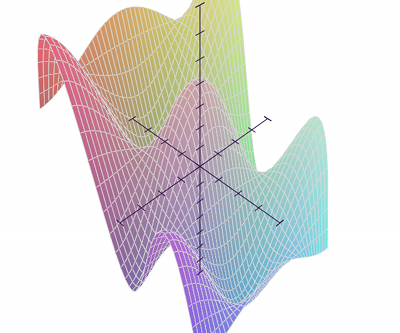
\includegraphics{plot.jpg}
\caption{Output of plotting example}
\end{figure}

\subsection{Supported Outputs}

SymPy supports within its printing and formatting utilities a variety of output formats ranging from pretty ASCII art to LaTeX and MathML. SymPy can also produce C and Fortran code as part of its printing and formatting capabilities. The C printer will try to use the standard C math libraries as much as possible. Of course, custom output formats can be implemented as well. Extending SymPy’s supported output formats will be discussed in the next section.

\subsection{Implementation}
SymPy’s formatting and printing implementation adheres tightly to an object oriented programming paradigm. At the root of the hierarchy, there is a base class called Printer that provides the infrastructure and boilerplate code that every formatting and printing implementation relies on. Such organization makes use of Python’s polymorphic features such as method overriding and dynamic dispatch while offering a neat and compact codebase to develop and debug on. Due to interoperability with legacy versions of SymPy, the printing framework is implemented in three parts:

1. The object prints itself:

Legacy versions of SymPy implemented printing as a method in every class. The Printer system will still execute any print method defined in a class before resorting to other methods.

2. Take the best fitting method defined in the printer:

An implementation’s subclass would implement the proper methods according to the interface specification in the Printer class.

3. As fallback, use the emptyPrinter method for the printer:

An implementation may not support printing certain expressions. In this case, fallback method with will be called to handle such expressions. If not implemented, the default emptyPrinter will be called from the parent class.

The steps to implementing a custom Printer can be summarized by the following steps:

1. Subclass the Printer class.

2. Define the Printer.printmethod method in the subclass.

3. Define the \_print\_CLASS methods in the subclass.

4. If convenient, override self.emptyPrinter in the subclass.

\end{document}
